\chapter{\label{ch:least squares solutions}Least Squares Solutions}

\section{\label{sec:ftola}Fundamental Theorem of Linear Algebra}  %    S    S    S    S    S    S    S    S    S    S    S    S  
\index{Fundamental Theorem of Linear Algebra!orthogonal decomposition}
\begin{table}[htbp]  %  T A B L E
    \caption[The Fundamental Theorem of Linear Algebra]{The Fundamental Theorem of Linear Algebra for $\aicmn$ }
    \begin{center}
    		\begin{tabular}{rlcccccccc}
    		  %
    		  domain:   & $\cmplx{n}$ & = & $\brnga{*}$ & $\oplus$ & $\rnlla{}$ \\
    		  %
    		  codomain: & $\cmplx{m}$ & = & $\brnga{}$  & $\oplus$ & $\rnlla{*}$
    		  %
      \end{tabular}
    \end{center}
  \label{tab:ftola}
  \end{table}%

  \begin{table}[ht]
    \caption[The Fundamental Theorem of Linear Algebra in pictures]{The Fundamental Theorem of Linear Algebra for $\aicmn$}
    \begin{center}
      \begin{tabular}{crclc}
          %
          Domain &&&& Codomain \\\hline
          %
          \ \\
          %
          $\cmplxn$ &&&& $\cmplxm$ \\[10pt]
          %
          \multirow{3}{*}{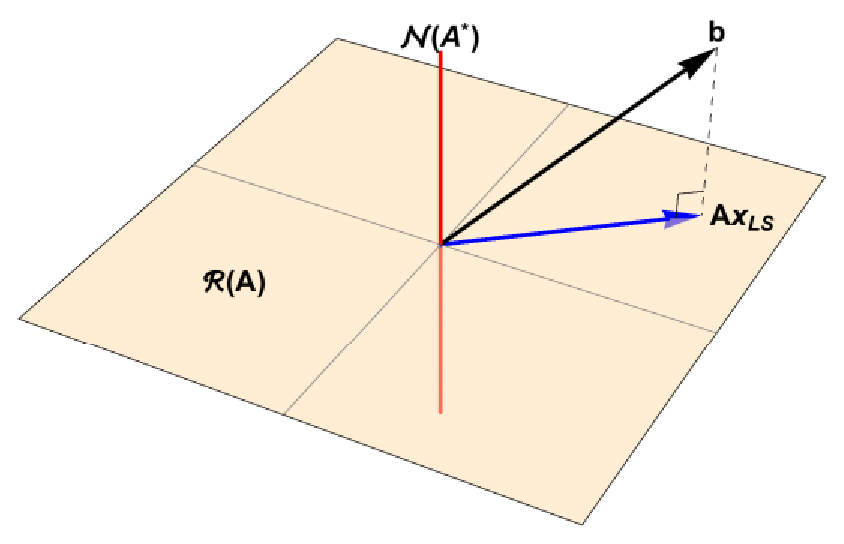
\includegraphics[ width = 1.7in ]{../graphics/ftola/domaingimp}} &&&&
          \multirow{3}{*}{\includegraphics[ width = 1.7in ]{../graphics/ftola/codomaingimp}} \\[5pt]
            & $\A{} \colon \cmplx{n}$ & $\mapsto$ & $\cmplx{m} $ \\[15pt] 
            & $\cmplx{n}$ & $\mapsfrom$ & $\cmplx{m} \colon \A{*}$ \\
          %
      \end{tabular}
    \end{center}
  \end{table}

\endinput